\documentclass{beamer}
\usetheme{Antibes}
\usecolortheme{beaver}
\usepackage{amsmath}
\usepackage[utf8]{inputenc}
\usepackage{tikz}

\def\insertauthorindicator{Who?}% Default is "Who?"
\def\insertinstituteindicator{From?}% Default is "From?"
\def\insertdateindicator{When?}% Default is "When?"

\title{Neural networks}
\subtitle{Architectures and training tips}

\author{Sebastian Bj{\"o}rkqvist}
\institute{IPRally Technologies}

\date[09.01.2019]{09.01.2019}

\newcommand{\kur}{\protect\textit}
\newcommand{\bol}{\protect\textbf}

\def\layersep{2.2cm}
\begin{document}

\frame{\titlepage}
  \begin{frame}
    \frametitle{What is a neural network?}  
    
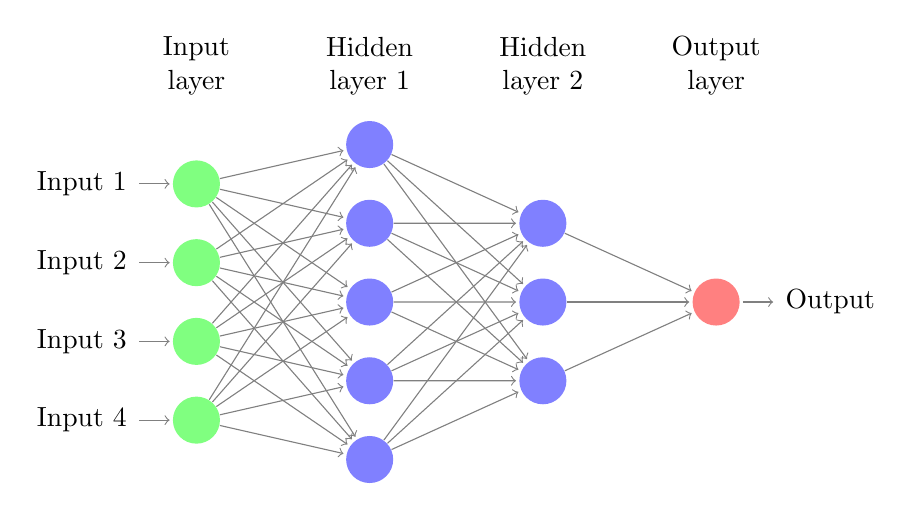
\begin{tikzpicture}[shorten >=1pt,->,draw=black!50, node distance=\layersep]
    \tikzstyle{every pin edge}=[<-,shorten <=1pt]
    \tikzstyle{neuron}=[circle,fill=black!25,minimum size=17pt,inner sep=0pt]
    \tikzstyle{input neuron}=[neuron, fill=green!50];
    \tikzstyle{output neuron}=[neuron, fill=red!50];
    \tikzstyle{hidden neuron}=[neuron, fill=blue!50];    
    \tikzstyle{hidden neuron 2}=[neuron, fill=blue!50];
    \tikzstyle{annot} = [text width=4em, text centered]

    % Draw the input layer nodes
    \foreach \name / \y in {1,...,4}
    % This is the same as writing \foreach \name / \y in {1/1,2/2,3/3,4/4}
        \node[input neuron, pin=left:Input \y] (I-\name) at (0,-\y) {};

    % Draw the hidden layer nodes
    \foreach \name / \y in {1,...,5}
        \path[yshift=0.5cm]
            node[hidden neuron] (H-\name) at (\layersep,-\y cm) {};

    % Draw the hidden layer nodes
    \foreach \name / \y in {1,...,3}
        \path[yshift=-0.5cm]
            node[hidden neuron 2] (F-\name) at (2*\layersep,-\y cm) {};

    % Draw the output layer node
    \node[output neuron,pin={[pin edge={->}]right:Output}, right of=F-2] (O) {};

    % Connect every node in the input layer with every node in the
    % hidden layer.
    \foreach \source in {1,...,4}
        \foreach \dest in {1,...,5}
            \path (I-\source) edge (H-\dest);
    \foreach \source in {1,...,5}
        \foreach \dest in {1,...,3}
            \path (H-\source) edge (F-\dest);

    % Connect every node in the hidden layer with the output layer
    \foreach \source in {1,...,3}
        \path (F-\source) edge (O);

    % Annotate the layers
    \node[annot,above of=H-1, node distance=1cm] (hl) {Hidden layer 1};
    \node[annot,right of=hl, node distance=\layersep] (fl) {Hidden layer 2};
    \node[annot,left of=hl] {Input layer};
    \node[annot,right of=fl] {Output layer};
\end{tikzpicture}

  \tiny Modified from \url{http://www.texample.net/tikz/examples/neural-network/}
  \end{frame}

  \begin{frame}
    \frametitle{Why neural networks?}  
    
   	\begin{itemize}
		\item Can approximate any function \cite{hornik}
		\item May learn to respond to unexpected patterns
		\item Useful especially when the amount of data is large
		\item Less need for feature engineering compared to traditional ML methods
	\end{itemize}
  \end{frame}

%   
   \begin{frame}
   	\frametitle{References}
   	\begin{thebibliography}{Hornik, 1991}

  \bibitem[Nielsen, 2015]{nielsen} Nielsen, Michael A. {\em Neural Networks And Deep Learning}. Determination Press, 2015. \url{http://neuralnetworksanddeeplearning.com/}
  
  \bibitem[Hornik, 1991]{hornik} Hornik, Kurt. {\em Approximation Capabilities of Multilayer Feedforward Networks}. Neural Networks, 4(2), 251--257, 1991.
    
	\end{thebibliography}   
   \end{frame}  

\end{document}
